\chapter{Struttura del progetto}
\label{cap:Struttutra_Progetto}
In questo capitolo mostro l'architettura software del progetto, mettendo in
evidenza i moduli di cui è composto e le varie relazioni che sussistono tra di loro.\\
Prima di tutto bisogna definire il concetto di modulo :     
       \begin{quote}
       \textit{``Un \textbf{modulo software} è una porzione di software, che
	contiene e fornisce servizi o risorse e a sua volta può usufruire di risorse o
	servizi offerti da altri moduli.\\ L'insieme dei servizi 
	messi a disposizione prende il nome di \textit{interfaccia}.''}
       \end{quote}

Si è deciso di adottare una struttura modulare per ottenere una maggior
chiarezza e una più semplice gestione del sistema file system. 
Ogni modulo è composto da una o più componenti, ognuna delle quali svolge un compito
ben preciso. \\ 
Il principale vantaggio di questo approccio è quello che,  qualora si volessero
introdurre delle modifiche, per ottenere miglioramenti o nuove funzionalità, queste riguarderebbero solo 
il modulo interessato senza che ciò comporti variazioni o malfunzionamenti sugli altri moduli.\\
Per esempio se uno volesse introdurre una cache delle scritture, questa modifica
riguarderebbe solamente il modulo a cui è stato assegnato il compito di gestire
la zona dati del disco, mentre gli altri moduli non 
subirebbero modifiche. 

\section{Struttura Modulare}
\label{sech:Struttura_Modulare}
Il File system è composto da tre macro-moduli, che riprendono la struttura
generale di un file sytem vista nel precedente capitolo §\ref{cap:FileSystem}. Seguendo un
approccio bottom-up descriviamo il funzionamento generale di questi moduli.
\begin{description}
 \item[Modulo Base]
    Il primo modulo è il modulo base. Lo scopo di questo modulo è di
interfacciarsi con il driver del disco e di fornire al modulo superiore un
interfaccia con la quale gestire le regioni FAT e Data del disco. 
 \end{description}
\begin{description}
 \item[Modulo Gestore File]
  Il secondo Modulo è il modulo intermedio, che esegue la gestione logica dei file.
  Si occupa della gestione entry FAT e dei nomi. Fornendo un'interfaccia
  semplice al modulo superiore mediante la quale si possono gestire i file tramite il concetto di file control block ( spiegato nel paragrafo §\ref{sez:Req} ).
 \end{description}
\begin{description}
 \item[Modulo File system logico]
 Mette a disposizione le system call usate dall'utente finale, e traduce le informazioni ottenute dall'utente in informazioni comprensibili ai livelli inferiori. 
 \end{description}
Sia le comunicazioni tra i vari moduli del sistema, sia le comunicazioni tra i moduli e i componenti esterni appartenenti al nucleo avvengono mediante opportune strutture dati.  
Ogni modulo conosce la struttura dati del modulo precedente e di quella del modulo successivo. \\
La figura \ref{Fig:StrutturaFS} riassume con semplicità questo concetto. 
Le strutture dati sono individuate dal nome posto sopra i link che collegano i vari moduli. Nei paragrafi successivi, le strutture dati verrano analizzate con un miglior detaglio.\\

\begin{center}
\begin{figure}[h]
 \centering
 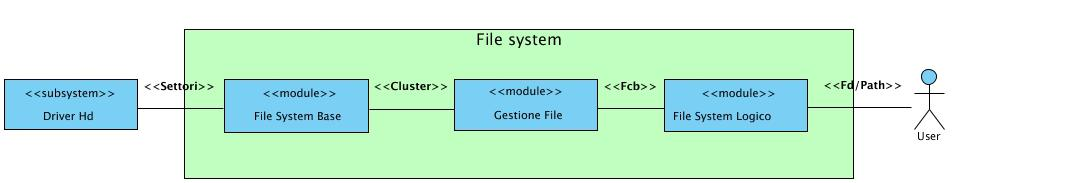
\includegraphics[width=400px,height=70px]{./Immagini/FS.jpg}
 % FS.jpg: 1070x183 pixel, 96dpi, 28.31x4.84 cm, bb=0 0 803 137
 \caption{Struttura generale del sistema.}
 \label{Fig:StrutturaFS}
\end{figure}\end{center}

\section{Modulo Base}
\label{sect:ModuloBase}
Il modulo base è il modulo che si occupa della gestione a basso livello del file system. Lo scopo è quello di gestire in modo corretto le zone dati e FAT del disco e di mostrare ai livelli superiori un'
interfaccia semplice con la quale interagire. 
Il compito di questo modulo rimane comunque molto complesso, si è perciò deciso di scomporlo in componeti più semplici a ciascuno dei quali è stato assegnato uno scopo specifico.\\
Di seguito verrano illustrati i singoli componenti. 
 
\subsection{Volume}
  Il primo componente chiamato dal sistema è il componente Volume. Questo ha il compito di analizzare il disco alla ricerca delle partizioni FAT. Una volta individuata crea la relativa struttura e la  inserisce nella tabella dei volumi. \\
  La \textit{tabella dei volumi} è una struttura globale, necessaria ai moduli superiori per una corretta gestione dei volumi presenti nei dischi. E' una struttura molto semplice realizzata mediante una lista concatenata nella quale vengono inseriti tutti i moduli rilevati. \\
  Per ogni volume sono presenti due semafori di mutua esclusione, uno riservato alla gestione della Regione Dati e l'altro per la Regione FAT.
  Sono inoltre presenti informazioni riguardanti la formattazione del volume, un puntatore alla FAT in memoria e un puntatore al FCB della root.\\

  Il modulo mette a disposizione la seguente interfaccia : \\	
    \begin{description}
     \item[crea\_tabella\_volumi]
    Questa funzione ha lo scopo di creare la tabella dei volumi.  La funzione per poter creare la tabella cerca nel disco mediante la primitiva di sistema get\_partizione le partizioni fat, una volta identificate crea  ed inserisce nella lista un nuovo elemento. Nell'elemento inserirà tute le informazioni attinenti a quel volume, assegnerà un etichetta univoca e creerà ed inizializzerà il FCB della root directory. \\
    \end{description}
    
    \begin{description}
     \item[print\_tabella]
	E' una funzione di debug, che viene usata per stampare a video il contenuto della tabella. \\
     \end{description}
     
    \begin{description}
     \item[get\_volume]
	 E' una funzione di utilità necessaria per rintracciare un determinato volume mediante l'etichetta. \\
     \end{description}
 
    \begin{description}
      \item[delete\_tabella]
	E' Funzione che viene chiamata esclusivamente in caso di errore per rilasciare le varie zone dati allocate.\\
     \end{description}

\section{Fat}	
  Il Secondo componente del modulo base è il componente FAT. Questo ha il compito di gestire in modo corretto la tabella FAT. A questo livello tutti i file vengono gestiti mediante le catene di cluster che sono salvate
  nella FAT. Quindi, il compito principale di questo componente è quello di offrire un'interfaccia semplice che permetta la creazione, la modifica e l'eliminazione di queste catene.\\
  Per questioni di efficienza si è scelto di caricare la tabella FAT in memoria, ciò comporta però un inconveniente, infatti la tebella FAT in memoria deve essere sempre in uno stato consistente con quella presente nel disco. Tutte le scritture devono comportare una scrittura sia nel disco e sia nella memoria e poiché si potrebbero verificare delle inconsistenze tra i dati le scritture devono avvenire in mutua esclusione tra loro. 
  Questa procedura è regolata dal semaforo presente nel volume associato alla tabella FAT corrispondente.\\

  Il modulo esporta la seguente interfaccia  : \\
   
  \begin{description}
   \item[delete\_memory\_fat] Funzione che elimina la tabella FAT dalla memoria solitamente usata in casi di errore.
  \end{description}
    \begin{description}
   \item[get\_next\_fat]Funzione utilizzata per scorrere una catena FAT. Questa funzione esegue dei controlli sulla consistenza della catena stessa.
  \end{description} 
    \begin{description}
   \item[init\_fat]Funzione che carica in memoria la tabella FAT.  
   \end{description}
  \begin{description}
   \item[create\_fat ] Funzione che crea una nuova catena FAT.
  \end{description}  
  \begin{description}
   \item[append\_fat]Funzione che aggiunge un cluster alla catena.
  \end{description}
  \begin{description}
   \item[delete\_fat]Funzione che elimina l'ultimo cluster dalla catena.
  \end{description}   
  \begin{description}
   \item[delete\_fat\_all]Funzione che elimina tutta la catena.
  \end{description}     
 \begin{description}
  \item[print\_chain] Funzione di debug che stampa a video la catena. 
  \end{description}     
    

\subsection{DATA}
\label{sec:Data}
  L'ultimo componente presente nel modulo base è il componente data, che ha lo scopo di gestire la zona dati. \\
  Questo componente mette a disposizione degli altri moduli le funzioni di scrittura e lettura sul disco.\\
  I moduli che usano queste funzioni devono fornire solamente la catena di cluster sulla quale si vuole scrivere e l'offset di scrittura, in questo modo si offre un visione
  uniforme dello spazio del disco, semplificando le operazioni di lettura e scrittura per i moduli superiori.\\
  
  Il modulo esporta la seguente interfaccia: 
    \begin{description}
     \item[write\_data] Funzione che scrive  sulla catena di cluster specificata come argomento, all'offset specificato.
     \end{description}
    \begin{description}
     \item[read\_data]  Funzione che legge sulla catena di cluster specificata come argomento, all'offset specificato.
    \end{description}
  Queste sono le uniche due funzioni che vengono usate per l'accesso ai dati nel disco. 

  \begin{figure}[!h]
 \centering
  \textheight 10px
 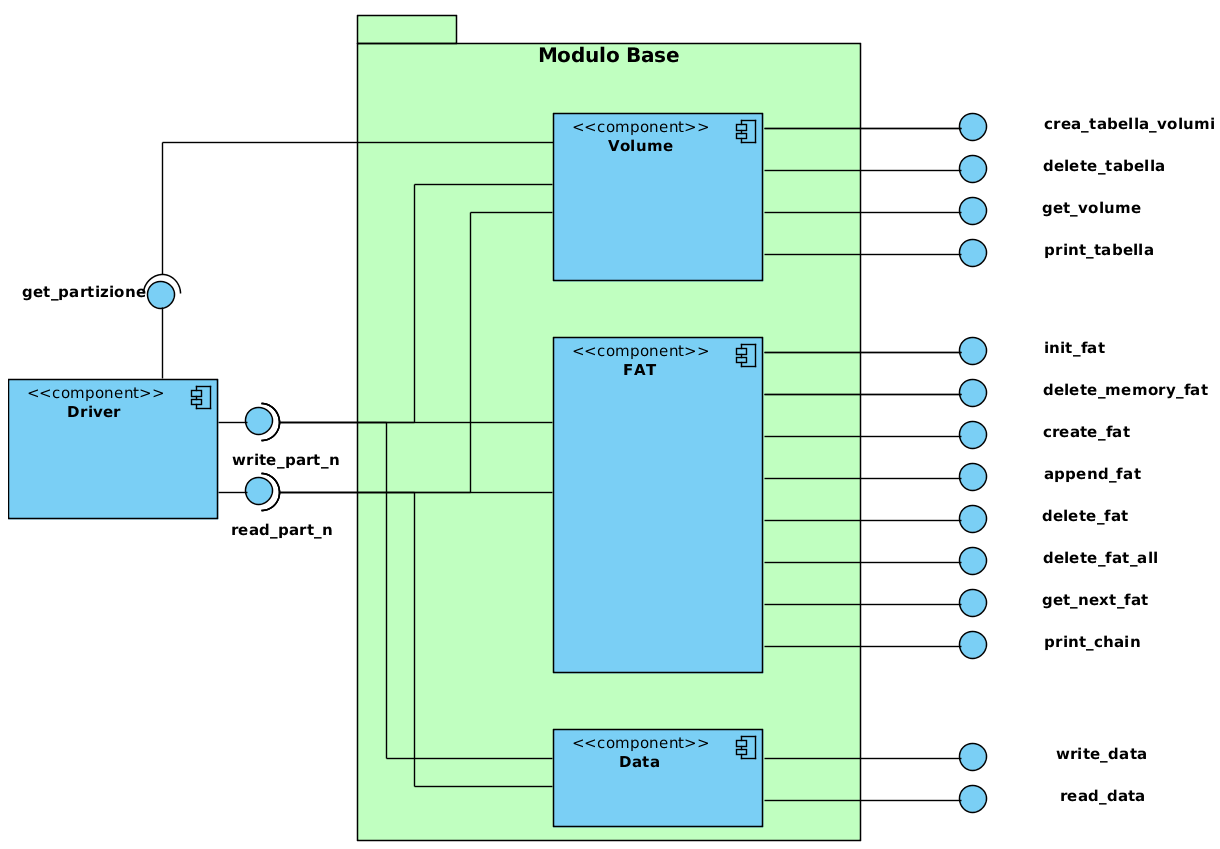
\includegraphics[width=400px,height=300px]{./Immagini/Base.png}
 % Base.png: 1220x849 pixel, 96dpi, 32.28x22.46 cm, bb=0 0 915 637
 \caption{Modulo Base}
 \label{fig:Base}
\end{figure}

\newpage 

\section{Modulo Gestore dei File}
 Il modulo Gestore dei file è il modulo che fa da intermediario tra il modulo base e quello logico.
  La funzionalità principale di questo modulo è quella di gestire i file e le cartelle. 
 Il modulo intermedio colloquia con il modulo logico mediante una struttura dati che prende il nome di \textbf{file control block (FCB)}. 
 Questa struttura è di fondamentale importanza per la gestione dei file, la tabella successiva ne riassume i vari campi.
  
\begin{center}
\begin{tabular}{|l|l|}\hline
\textbf{Campo} & \textbf{Significato}\\\hline
volume & Puntatore al volume nel quale è presente il file\\\hline
cluster & Numero del primo cluster\\\hline
type & Flag presente nella short entry\\\hline
mode & Modalita di apertura\\\hline
pos\_corr & Posizione corrente nel file\\\hline
size & Grandezza del file\\\hline
cluster\_father & Cluster della direcotory nel quale inserito\\\hline
offset\_father & Offset all'interno della directory\\\hline
n\_entry & Numero entry di cui è composto\\\hline
\end{tabular}
\end{center}

È la struttura nella quale sono presenti tutte le informazioni necessarie per la gestione dei file. \\

  \subsection{Direntry}
    Il componente direntry, è il componente principale di questo modulo. Lo scopo di questo componente è quello di gestire le strutture dati che contengono le informazioni dei file. 
    Nella gestione delle entry dei file si sono seguite le specifiche Microsoft in modo pedissequo. \\
    Il sistema è in grado di rilevare e gestire in maniera corretta file formati da entry lunghe più entry corte, file formati da sole entry corte (vedi \ref{gest:dir}). \\
    Si è prestato particolare cura nella realizzazione dell'algoritmo per la generazione dei nomi corti. In particolare nel caso di nomi simili\footnote{Per il concetto di Nomi simili si intendono nomi uguali per i primi 8 caratteri.},
   l'algoritmo genera il numero corretto, controllando che nel disco non sia già presente un file con quel nome. Nel caso si arrivi alla presenza di 10 file con i nomi simili nella stessa cartella, il sistema 
   genererà il nome corto in modo casuale. \\
  L'interfaccia esportata da questo modulo è la seguente : 

    \begin{description}
     \item[open\_entry]
     Funzione che effettua la ricerca di un file e se presente inizializza il FCB associato. 
     \end{description}

    \begin{description}
     \item[delete\_entry]
      Funzione che elimina un entry. Se presente una catena di cluster associata all'entry oggetto dell'eliminazione, anche questa verrà rimossa. 
     \end{description}
   
    \begin{description}
      \item[create\_entry]
      Funzione che crea un entry ed inizializza il FCB associato. 
    \end{description}

    \begin{description}
     \item[rename\_entry]
      Funzione che modifica il nome di un entry. Modifica opportunamente il FCB associato.   
   \end{description}

    \begin{description}
     \item[create\_directory]
      Funzione che crea una directory vuota. Inizializza in modo opportuno il FCB associato. 
     \end{description}

    \begin{description}
     \item[delete\_directory]
      Funzione che elimina una directory vuota. 
     \end{description}
  

  \subsection{FCB}
    Questo componente è molto semplice, contiene la definizione della struttura dati FCB vista precedentemente. Inoltre in questo componente ho inserito le funzioni che permettono la scrittura e la lettura
    usando i FCB per individuare  il file o la directory.  Il loro compito e solo quello di estrarre le informazioni dal FCB , chiamare le funzioni read\_data e write\_data presenti nel modulo inferiore e 
    aggiornare se necessario i campi del FCB. 
  
  \newpage

  \begin{figure}[h]
 \centering
 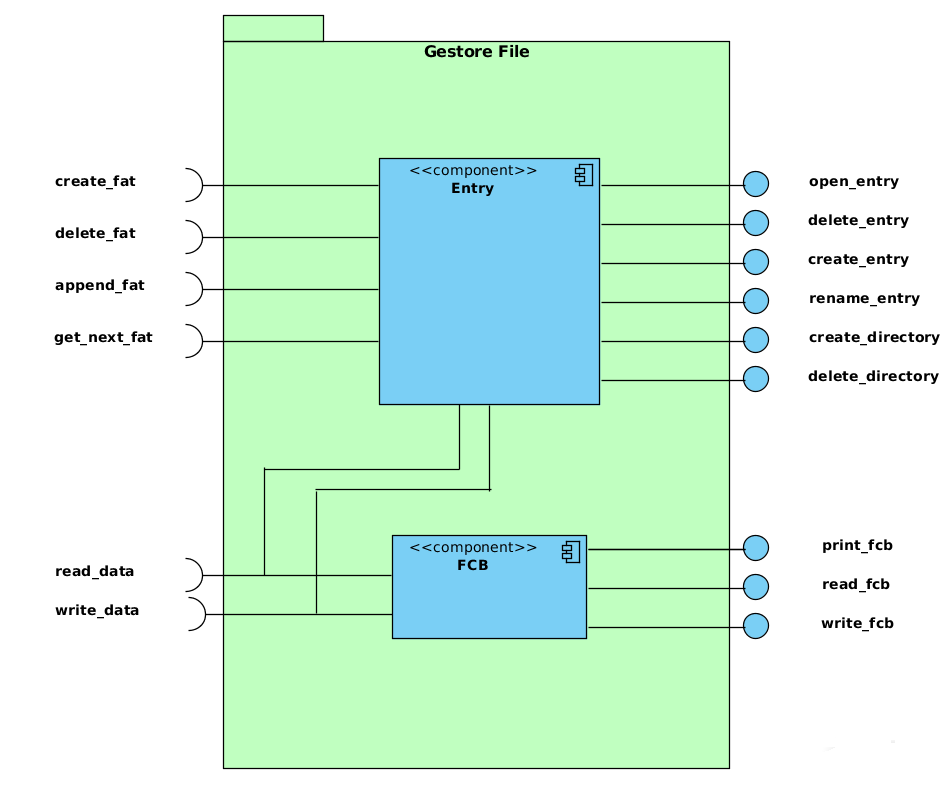
\includegraphics[width=400px,height=350px]{./Immagini/GestoreFile.png}
 % GestoreFile.png: 949x788 pixel, 96dpi, 25.11x20.85 cm, bb=0 0 712 591
 \caption{Gestore File}
 \label{fig:GestoreFile}
\end{figure}


\section{System Call}
\label{sec:Logico} 
   Il modulo system call è il modulo che implementa tutte le system call esportate a livello utente. \\		
   Il compito principale di questo modulo è quello di elaborare le informazioni ottenute dall'utente ed inizializzare gli opportuni Fcb con i quali chiamare le funzioni del livello precedente. 
   Un ulteriore compito di questo è quello di gestire le aree di memoria riservate nel modulo sistema necessarie per il salvataggio delle informazioni private per ogni processo, mediante le primitive viste nel paragrafo § \ref{AreaPrivataProcesso}.\newpage
   L'interfaccia esportata da questo modulo coincide con le system call appartenenti al file system : \\
          
     
     \begin{description}
      \item[open]
	System call che apre il file specificato dall'utente. Si occupa di creare il relativo FCB ed inserirlo nell'area privata del processo.
	Riporta il file descriptor associato al file oggetto della chiamata.\\
	Il file può essere aperto nelle seguenti modalità : \\
	  \begin{itemize}
	   \item O\_RDONLY   :   apre il file in sola lettura.\\			
 	   \item O\_WRONLY   :   apre il file in sola scrittura.\\				
 	   \item O\_RDWR     :   apre il file in lettura/scrittura.\\			
 	  \item  O\_CREAT    :   se il file non esiste verrà creato.\\			
 	   \item O\_DIRECTORY :   se il path specificato non è una directory la chiamata fallisce  \\ 
       \end{itemize}
     \end{description}
      
      \begin{description}
       \item[close]
	System call che chiude il file specificato dall'utente mediante il file descriptor. Inoltre rimuove il Fcb associato al file oggetto della chiamata.
       \end{description}
       
       \begin{description}
        \item[read] System call usata per leggere i dati da un file. Il file deve essere stato precedentemente aperto.
       \end{description}

        \begin{description}
         \item[write] System call usata per scrivere i dati su un file. Il file deve essere stato precedente aperto. 
         \end{description}

     \begin{description}
      \item[lseek] System call usata per spostare la posizione corrente su un file.Il file deve essere stato precedentemente aperto. 
      Si può inoltre indicare il punto di partenza dal quale inserire l'offset usando i seguenti parametri : \\
	\begin{itemize}
	 \item SEEK\_SET si fa riferimento all'inizio del file,  
	      il valore (sempre positivo) di offset indica direttamente la nuova posizione corrente.        
	 \item SEEK\_CUR si fa riferimento alla posizione corrente del file,  ad essa viene sommato offset (che può essere negativo 
	      e positivo) per ottenere la nuova posizione corrente. 
	\item  SEEK\_END si fa riferimento alla fine del file, alle dimensioni  del file viene sommato offset (che può essere negativo  e positivo) per ottenere la nuova posizione corrente.  
	\end{itemize}

      \end{description}
    
    \begin{description}
     \item[remove] System Call il cui scopo è rimuove un file. Il file non deve essere stato aperto in precedenza. 
     \end{description}
     
     \begin{description}
      \item[rename] System Call il cui scopo è rinominare un file.Il file non deve essere stato aperto in precedenza. 
      \end{description}

    \begin{description}
     \item[mkdir]System call il cui scopo è di creare una directory.
     \end{description}
     
     \begin{description}
      \item[rmdir] System call il cui scopo è di eliminare una directory, solamente se questa è vuota. 
      \end{description}
      
      \begin{description}
       \item[chdir] System call il cui scopo è di modificare la directory corrente associata al processo. 
       \end{description}

      \begin{description}
     \item[getcwd] System call il cui scopo è di riportare la directory corrente associata la processo. 
    \end{description}
  
\begin{figure}[h]
 \centering
 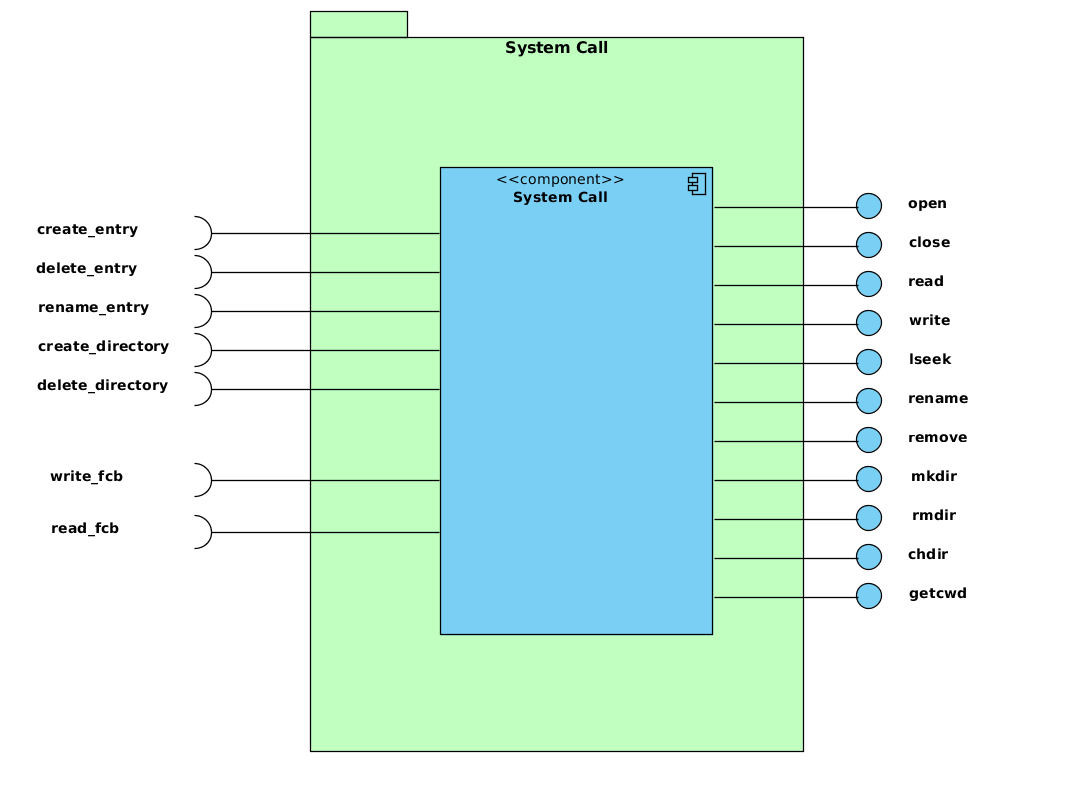
\includegraphics[width=350px,height=280px]{./Immagini/system_call.png}
 % system_call.png: 1084x788 pixel, 96dpi, 28.68x20.85 cm, bb=0 0 813 591
 \caption{ Modulo SystemCall}
 \label{fig:SystemCall}
\end{figure}


\section {Processo di Inizializzazione}
   Il processo di inizializzazione non è un modulo come quelli presentati precedentemente. Ho scelto di inserirlo in questa sezione poiché ricorrerò ai concetti presentati nei paragrafi precedenti. 
  
   E' rappresentato dalla funzione \textbf{fs\_init}, che ha il compito di inizializzare il file system. 
   Questa funzione invoca le funzioni di inizializzazione dei moduli. La prima azione che viene eseguita è la creazione della tabella dei volumi, successivamente vengono caricate in memoria le tabelle FAT dei vari volumi ed infine viene inizializzata l'area privata del processo di IO. L'inizializzazione dell'area privata del processo di IO, fa sì che tutti i suoi processi figli ereditino le informazioni dal padre.\\ 
  
\section {Conclusioni}
  In questo capitolo abbiamo presentato la struttura generale del sistema, mettendo in evidenza i vari moduli, componenti e interfacce mediante le quali colloquiano.
  Non ci siamo addentrati nei dettagli implementativi, per questi si rimanda ai sorgenti del sistema, che sono accompagnati da una discreta quantità di commenti per agevolarne la comprensione. 
  
\clearpage{\pagestyle{empty}\cleardoublepage